\documentclass[12pt,oneside]{book}

\usepackage{ulamonog} %proyecto de grado
%\usepackage[ansinew]{inputenc} % escribir acentos
\usepackage[utf8]{inputenc}

%\usepackage[activeacute,spanish]{babel}
\usepackage{moreverb}
%\usepackage{url}
\usepackage{cite}

\usepackage{graphicx}
\usepackage{float}
\usepackage{listings}
\usepackage{pdflscape} 
\usepackage{fancyvrb}
\usepackage{fancybox}
\usepackage{enumerate}
\usepackage{lmodern}
\usepackage[T1]{fontenc}


\usepackage{color}
\usepackage[colorlinks]{hyperref}
\usepackage[spanish]{babel}
\selectlanguage{spanish}
\usepackage[utf8]{inputenc}
\usepackage[numbers,sort]{natbib}
\setcounter{secnumdepth}{4}
\setcounter{tocdepth}{4}
% ***************************************************************** %
% En el siguiente comando se pueden modificar (para el archivo .pdf):
% Titulo, Autor, Palabras clave
% ***************************************************************** %

% si se va a imprimir,
% se incluye al final despues de citecolor=blue, el comando draft=true
\hypersetup{pdftitle={Título de prueba: si es de verdad},
	pdfauthor={Autor},
	pdfsubject={Proyecto de Grado}, % se deja igual
%	pdfkeywords={Palabras,claves,muchas,pocas},
	 pdfstartview=FitH,bookmarks=true,
	  citecolor=blue, draft=true}

% Si desea que no aparezca la lista de tablas o figuras descomente las siguientes lineas
\nolistoftables
\nolistoffigures

% ***************************************************************** %
% FIN DE
% Titulo, Autor, Palabras clave
% ***************************************************************** %


\sloppy
\begin{document}
	
	\frontmatter
	
	
	% ***************************************************************** %
	% Si sabe la fecha de presentación del Proyecto de Grado
	% con o sin comentar
	% ***************************************************************** %
	%\fechaentrega{Junio} % Si sabe cuando se presentó
	%\presentaciondia{2 de Junio} % si conoce exactamente el día
	%\presentacionlugar{Laboratorio 226 de EISULA} % si conoce exactamente el lugar donde se presentó
	% ***************************************************************** %
	% FIN DE
	% Si sabe la fecha de presentación
	% ***************************************************************** %
	
	% ***************************************************************** %
	% Si el Proyecto de Grado tiene mencion especial
	% con o sin comentar
	% ***************************************************************** %
	%\mencionespecial{Este proyecto fue seleccionado como \textbf{mejor proyecto de grado} de la Escuela de
	%Ingeniería de Sistemas, en el IC aniversario de la Facultad de Ingeniería.} % si tiene mención especial
	% ***************************************************************** %
	% FIN DE
	% Si sabe la fecha de presentación
	% con o sin comentar
	% ***************************************************************** %
	
	
	% ***************************************************************** %
	% Portada y resumen
	% ***************************************************************** %
	% Si desea el logo en la parte de abajo
	%\logoabajo
	
	% En caso de que el año sea diferente al actual, quite el comentario a la siguiente linea
	%\copyrightyear{2007}
	
	% Al final cuando hayan presentado, sin comentar
	% deberia ser el número de tesis presentada y la opción, IO por ejemplo
	% Numero del proyecto
	%\numproy{00IO}
	
	% Puede cambiar el tipo de monografía, por defecto: Proyecto de Grado
	%\tipomonografia{Informe Final de Proyecto de Grado}
	
	% En caso de hacer propuesta de proyecto, quitele el comentario a la
	% siguiente linea --- En este caso no aparece ni la hoja de presentacion
	% ni la hoja de dedicatoria
	%\propuesta
	
	% Si se utiliza este formato para hacer un informe técnico, descomente las siguientes líneas
	\informe %
	\proyecto{} 
	% Datos del proyecto de grado
	\title{Migración y optimización del sistema Proceso Electoral}
	
	\author{Katherine Andrade}
	
	\cedula{20.199.494}
	\tutor{Ing. José Hidalgo}
	%\cotutor{Dra. Puede Haber}
	%\primerjurado{Dr. Primer Profesor}
	%\segundojurado{Prof. Segundo Profesor}
	% \tercerjurado{Prof. Tercer Profesor}
	
	% NO TOCAR si es Ingenieria de Sistemas

	
	%\signaturepage ----- NO TOCAR
	
	\resumen{El presente informe tiene como objetivo dar a conocer
		de   manera   concisa   y   clara   las   actividades   realizadas em Ogangi
		durante el periodo de las pasantías industriales cortas. Estas tuvieron una duración
		de ocho (8) semanas. \\
		En este periodo se desarrollaron actividades tales como la creación de las entidades por medio de Hibernate,la creación de la clase que permite la migración de Oracle a Postgresql, la modificación del código del proyecto utilizando todos los conocimientos aprendidos durante la carrera. Para realizar estas actividades se utilizó JAVA, el cual es un lenguaje de programación orientado a Objetos y también se hizo uso de la metodología ágil SCRUM la cual ayudo a tener avances semanales.\\
		 Todo esto se realizo junto al tutor industrial el cual siempre estuvo presente para aclarar las dudas que se iban presentando a medida que se avanzaba en el proyecto.
}
	
	
	\descriptores{Pasantías, SCRUM, Programación Orientada a Objetos, Hibernate, migración}
	
	%\cota{IXD A01.1}
	
	% Si es control y automatizacion se comenta la siguiente linea
	\opcion{Sistemas Computacionales}
	
	% ***************************************************************** %
	% FIN DE
	% Portada y resumen
	% ***************************************************************** %
	
	\beforepreface
	\listoffigures
	
	% ***************************************************************** %
	% Agradecimientos y primer capitulo (sin numeracion)
	% ***************************************************************** %
	%\prefacesection{Agradecimientos}
	
	%En esta sección se agradece a las personas que contribuyeron a llevar a buen final este trabajo.
	
	%%% Capitulo sin numero, antes de la pagina 1
	\prefacesection{Introducción}
	%Un párrafo de introducción al área de trabajo (4 líneas)
	
	En los últimos años, ha habido un interés creciente en el uso de las tecnologías para la comercialización de productos, haciendo que las empresas estén siempre buscando la manera eficiente de vender los mismos. Para lograr esto, se contratan empresas que se dediquen al desarrollo de tecnologías que permitan cumplir con los objetivos deseados. Ogangi es una empresa que ofrece ese tipo de servicios. \\
	
	El objetivo de la realización de este proyecto es optimizar código del sistema. Análisis, diseño e implementación de un módulo de Hibernate para el manejador de base de datos.  
	
	Ahora bien, para poder llevar a cabo el cumplimiento del objetivo, se necesita de conocimientos obtenidos en el transcurso de la carrera. Estos conocimientos se explican brevemente dentro de este informe 
	
	Finalmente, es conveniente acotar la configuración del presente documento, el cual ha sido organizado de la siguiente manera: Capitulo I, marco de referencia, Misión y Visión de la empresa; capitulo II, bases teóricas; capitulo III, aspectos procedimentales, plan de trabajo, desarrollo del plan y vinculación del proyecto con las materias de la carrera; conclusiones, anexos y bibliografías.
	
	\afterpreface 
	
	\pagestyle{fancyplain}
	\renewcommand{\chaptermark}[1]{\markboth{#1}{\textsc{\footnotesize\thechapter\ #1}}}
	\renewcommand{\sectionmark}[1]{\markright{\textsc{\footnotesize\thesection\ #1}}}
	\lhead[\fancyplain{}{\textsc{\footnotesize\thepage}}]%
	{\fancyplain{}{\rightmark}}
	\rhead[\fancyplain{}{\leftmark}]%
	{\fancyplain{}{\textsc{\footnotesize\thepage}}} \cfoot{}
	
	\mainmatter
	
	\chapter{Marco de Referencia}
	%Referencia a todos los trabajos (\emph{Recientes, < 4 años})

	Ogangi de Venezuela, C.A entrega millones de transacciones a través de las redes de
	datos móviles de América a través de su plataforma y actualmente procesa más de un millón de
	mensajes diarios, con sistemas informáticos redundantes, tolerante a fallas y con soporte las 24
	horas del día, por 7 días a la semana, los 365 días del año.	
	
	\section{Misión:}
	Su Misión está representada por la siguiente afirmación:
	“La tecnología de software y propiedad intelectual de Ogangi acelera y facilita la evolución
	de servicios móviles de datos. Permite a los operadores celulares crecer más rápidamente su
	oferta de servicios, a los proveedores y dueños de contenido de crear una presencia móvil, y a
	los usuarios móviles de gozar de los servicios a través de una experiencia satisfactoria”.
	
	\section{Visión:}
	“Los teléfonos, redes y servicios de datos de la telefonía móvil continuarán madurando y
	evolucionando hasta consolidarse como un medio de comunicación más comparable a los
	medios tradicionales como televisión y más recientemente Internet. La conveniencia de la
	ubicuidad y flexibilidad de los servicios móviles de datos permitirá a este nuevo medio inclusive
	integrar varios de los tradicionales”. \\
	
	En la actualidad, el negocio de Ogangi se divide principalmente en tres áreas:

\begin{itemize}
	
	\item Mensajería corporativa.	 
	\item Descarga de contenidos por medio de portales WAP y WEB. 	 
	\item Desarrollo de aplicaciones móviles. 	 
\end{itemize}

	De las tres áreas mencionadas, la mensajería corporativa ha sido el negocio principal de Ogangi desde sus inicios. Es por eso que año tras año, y juntos con los avances tecnológicos y tendencias en el mercado, Ogangi ha ido enriqueciendo su plataforma de mensajería, ofreciendo a sus clientes cada vez más canales para la entrega de información. \\
	
	Ogangi cuenta con una solución de mensajería interactiva que le permite a los usuarios obtener información referente al votante en un proceso electoral. \\
	Básicamente el cliente(compañía, empresa, etc) encargado del proceso proporciona los datos de los votantes a Ogangi, los cuales son insertados en una base de datos a través de un script, para ser consultados via SMS por los votantes.
	
	Las pasantías fueron realizadas específicamente en el área de desarrollo. Donde se realizo la actualización del proyecto que hace posible el envío de mensajes para obtener información referente al votante en un proceso electoral.

	\chapter{Bases Teóricas}
	
	\section{Programación Orientada a Objetos:}
	
	La programación orientada a objetos es un paradigma de programación que usa los objetos en sus interacciones, para diseñar aplicaciones y programas informáticos. \\
	
	
	Los objetos son entidades que combinan estado (atributo), comportamiento (método) e identidad.
	
	El estado de un objeto se refiere al conjunto de atributos y sus valores en un instante de tiempo dado. El comportamiento de un objeto puede modificar el estado de este.\\
	
	Dicho comportamiento, está directamente relacionado con su funcionalidad y determina las operaciones que este puede realizar o a las que puede responder ante mensajes enviados por otros objetos. \\
	
	La identidad, es la propiedad que permite diferenciar a un objeto y distinguirse de otros. Generalmente esta propiedad es tal, que da nombre al objeto. \\
	
	Este tipo de programación, está basada en varias técnicas, incluyendo herencia, cohesión, abstracción, polimorfismo, acoplamiento y encapsulamiento.\\
	
	Su uso se popularizó a principios de la década de los años 1990. En la actualidad, existe variedad de lenguajes de programación que soportan la orientación a objetos.
	
	\section{JAVA:} 
	
	Java es un lenguaje de programación orientado a objetos y es multiplataforma, ya que se puede ejecutar un mismo código en cualquier SO gracias a que se utiliza un entorno de ejecución de JAVA llamado JRE.
	Este lenguaje fue desarrollado por Sun Microsystems, posteriormente adquirido por Oracle. En la actualidad puede utilizarse de modo gratuito, pudiéndose conseguir sin problemas un paquete para desarrolladores que oriente la actividad de programar en este lenguaje. \\
	
	Puede ser modificado por cualquiera, circunstancia que lo convierte en lo que comúnmente se denomina “código abierto”.
	
	\section{Procedimientos almacenados:}
	
	Un procedimiento almacenado es un programa almacenado físicamente en una base de datos.
	Este programa al ser ejecutado en respuesta a una petición de usuario, es ejecutado directamente en el motor de la base de datos, el cual usualmente corre en un servidor separado. Como tal, posee acceso directo a los datos que necesita manipular y sólo necesita enviar sus resultados de regreso al usuario, deshaciéndose de la sobrecarga resultante de comunicar grandes cantidades de datos salientes y entrantes. \\
	
	La mayor parte de las veces, se utilizan para encapsular procesos complejos que podrían requerir  la ejecución de varias consultas SQL, tales como la manipulación de un conjunto de datos enorme para producir un resultado resumido. \\
	
	También pueden ser usados para el control de gestión de operaciones, y ejecutar procedimientos almacenados dentro de una transacción de tal manera que las transacciones sean efectivamente transparentes para ellos. \\
	
El hecho de que corra en un servidor separado, aumenta la rapidez de procesamiento de las peticiones del usuario. Los procedimientos almacenados pueden permitir que la lógica del negocio se encuentre como un API en la base de datos, que pueden simplificar la gestión de datos y reducir la necesidad de codificar la lógica en el resto de los programas cliente. Esto puede reducir la probabilidad de que los datos se corrompan por el uso de programas clientes defectuosos o erróneos. De este modo, el motor de base de datos puede asegurar la integridad de los datos y su consistencia con la ayuda de procedimientos almacenados.

	
	
	\section{Hibernate:}
	
	Hibernate es una herramienta de Mapeo objeto-relacional, esto quiere decir, que facilita el mapeo de atributos entre una base de datos relacional tradicional y el modelo de objetos de una aplicación, mediante archivos declarativos (XML) o anotaciones en los beans de las entidades que permiten establecer estas relaciones. \\
	Está diseñado para ser flexible en cuanto al esquema de tablas utilizado, para poder adaptarse a su uso sobre una base de datos ya existente. También tiene la funcionalidad de crear la base de datos a partir de la información disponible. \\
	
	Hibernate es software libre, distribuido bajo los términos de la licencia GNU LGPL.
	

	
	\section{Sistema de Gestor de Base De Datos(SGBD):}
	
	Es un conjunto de programas no visibles que administran y gestionan la información que contiene una base de datos. A través de él se maneja todo acceso a la base de datos con el objetivo de servir de interfaz entre ésta, el usuario y las aplicaciones.  \\
	
	En este proyecto, se utilizaron dos SGBD los cuales fueron: Oracle y Postgresql. \\
	
	Oracle, es un sistema de gestión de base de datos relacional (o RDBMS por el acrónimo en inglés de Relational Data Base Management System), fabricado por Oracle Corporation.\\
	
	Tradicionalmente, Oracle ha sido el SGBS por excelencia, considerado siempre como el más completo y robusto. Este SGDB siempre ha sido considerado de los más caros, por lo que no se ha estandarizado su uso como otras aplicaciones. \\
	
	Postgresql, es un sistema de gestión de base de datos relacional orientada a objetos y libre, publicado bajo la licencia BSD. \\
	
	Como muchos otros proyectos de código abierto, el desarrollo de PostgreSQL no es manejado por una empresa y/o persona, sino que es dirigido por una comunidad de desarrolladores que trabajan de forma desinteresada, libre y/o apoyada por organizaciones comerciales. La comunidad PostgreSQL se denominada el PGDG (PostgreSQL Global Development Group).



 %\citep{Wei}.\\
	
	%Mismo estilo para números y títulos
	
	
	\chapter{Aspectos Procedimentales}
	
	\section{Plan de trabajo:}
	
	El proyecto a desarrollar consiste en el levantamiento de información y el análisis del sistema previamente mencionado para posteriormente implementar los mecanismos que permitan finalizar con un producto mas robusto. \\
	
	Adicionalmente, se debe realizar el levantamiento de información, análisis, diseño e implementación de un modulo de Hibernate para el manejo de base de datos.
	
	\begin{itemize}
		
		\item Objetivos de las pasantías:	 
		\begin{itemize}
			\item Objetivo General:
			\begin{itemize}
				\item Optimizar código del sistema. Análisis, diseño e implementación de un módulo de Hibernate para el manejador de base de datos. 
			\end{itemize}
			\item Objetivos Específicos: \\
			Entre Los objetivos específicos que permitirán que se cumpla con el objetivo general, están:
			
			\begin{itemize}
				\item Revisión y comprensión de los componentes que conforman la solución actual para el sistema.
				\item Diseño e implementación de mejoras a los métodos presentes en el sistema.
				\item Diseño e implementación de un módulo de Hibernate para la gestión de base de datos.
				\item Actualizar el JDK a la última versión estable.
				\item Pruebas funcionales del sistema.
			\end{itemize} 
		\end{itemize}
		
	\end{itemize}
	
	En el siguiente Diagrama se puede apreciar el plan de trabajo propuesto por la empresa para las 8 semanas de pasantías y el desarrollo del plan.
	
	\begin{figure}[htb]
		\centering
		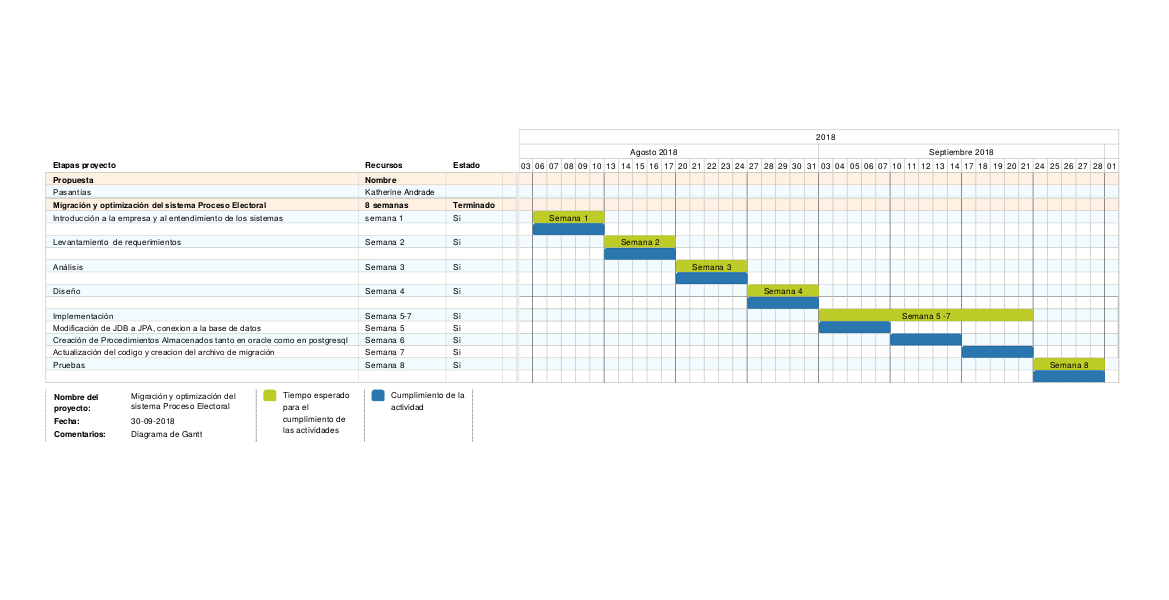
\includegraphics[width=1.1\textwidth]{diagrama1.png}
		\caption{Diagrama de Gantt}
		\label{i1}
	\end{figure}
	
	\break 
	\section{Desarrollo del plan:}
	\subsection{Introducción a la empresa y al entendimiento de los sistemas:}
	Semana dedicada a la introducción sobre la implementación actual del sistema, presentada por el Líder de desarrollo José Hidalgo. Explicación del Proyecto que se va a actualizar. \\
	
	Entrega de una computadora en la cual se realizara dicho proyecto.
	Instalación de los diferentes proyectos y herramientas a utilizar. \\
	
	Pruebas simples de las diferentes herramientas necesarias para poder llevar a cabo el proyecto de pasantías, con el fin de entender bien el manejo de dichas herramientas.
	
	\subsection{Levantamiento de Requerimientos:}
	Lograr el funcionamiento del proyecto basado en una conexión JPA. Crear las entidades en Hibernate con el fin de facilitar la migración de la base de datos, ya que hibernate permite la migración a cualquier gestor de base de datos.\\ 
	
	Creación de las entidades en Hibernate. Se selecciono una clave primaria para cada entidad, ya que a pesar de que la BD original es relacional, esta no contaba con las mismas. \\
	
	Hibernate no permite crear entidades sin claves primarias. Por lo tanto, se escogió para la mayoría de las tablas una clave primaria autoincremental.\\
	
	Creación del archivo XML para poder realizar el mapeo. 
	
	
	\subsection{Análisis:}
	Modificación de las funciones que se encuentran en la clase CNEUtil, las cuales son las utilizadas para realizar las consultas a la BD que se encuentra en Oracle por medio de una conexión JDBC.Estas fueron modificadas a JPA y su conexión se realiza por medio de Hibernate.\\

	Creación de Procedimientos Almacenados en Oracle de las consultas que se realizaban por medio de JDBC. \\
	
	Comienzo de la clase con la cual se realizara la migración de Oracle a Postgresql.
	
	\subsection{Diseño:}
	
	Creación de las tablas en Postgresql por medio del mapeo objeto-relacional. Esta creación se hizo en el servidor local. También se realizó la creación de los mismos Procedimientos Almacenados que se encuentran en Oracle, ya que estos funcionan correctamente.\\  
	
	Culminación de la clase Migrate, la cual es la encargada de realizar la migración de Oracle a Postgresql.
	
	\subsection{Implementación:}
	
	Modificación de las funciones de las clases Updater y getDBDataTest. Cambio de JDBC a JPA. Las consultas se realizaron por medio de Procedimientos almacenados.\\
	
	La clase Updater consta de funciones encargadas de insertar valores en una tabla especifica, actualizar o eliminar valores repetidos de la misma. La clase getDBDataTest hace una búsqueda en la BD de una cédula con el fin de probar que la conexión es exitosa.
	
	\subsection{Pruebas:}
	Realización de la migración de Oracle a Postgresql.\\
	
	Envío de un mensaje de texto para probar el funcionamiento del proyecto conectado con la BD remota que se encuentra en Oracle luego de terminar todas las modificaciones del proyecto.
	
	\begin{figure}[H]
		\centering
		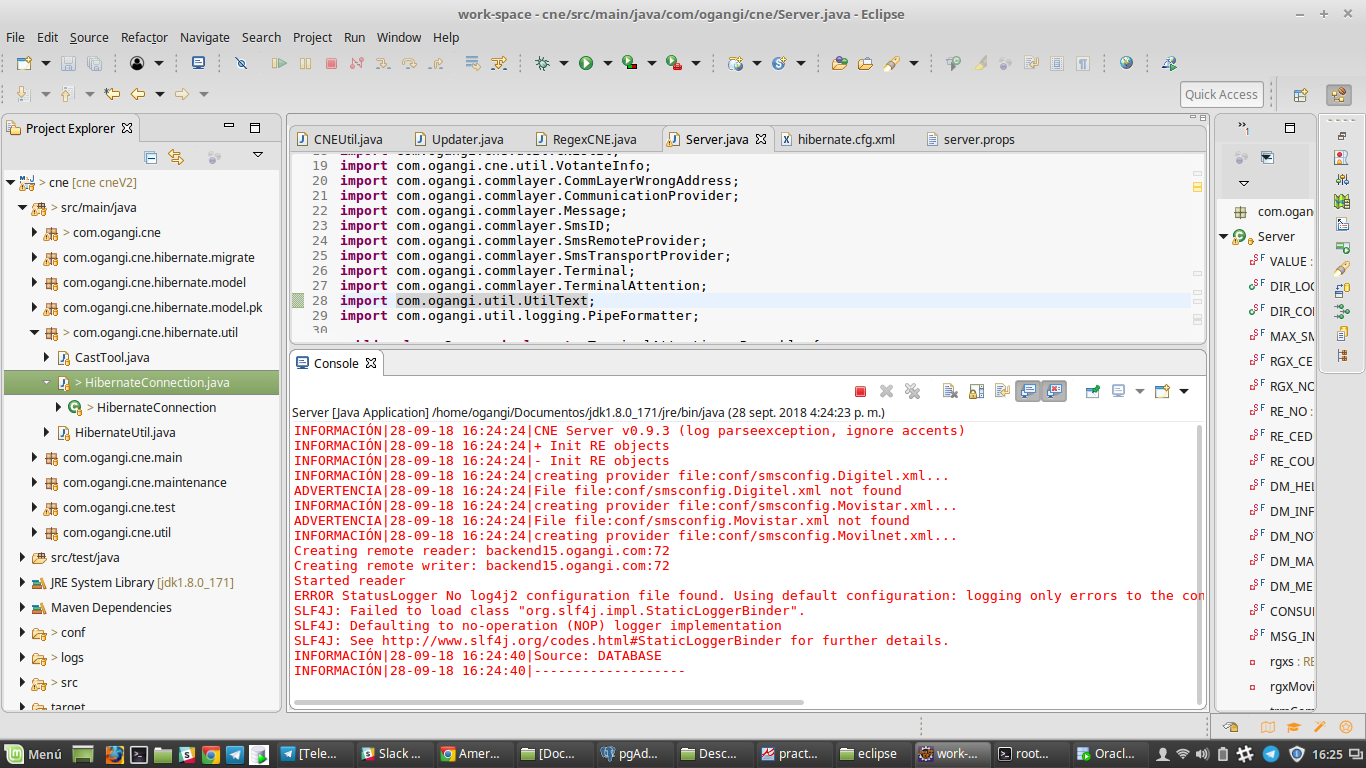
\includegraphics[width=0.8\textwidth]{conexion.png}
		\caption{Corriendo el servidor}
		\label{u1}
	\end{figure}


\begin{figure}[H]
	\centering
	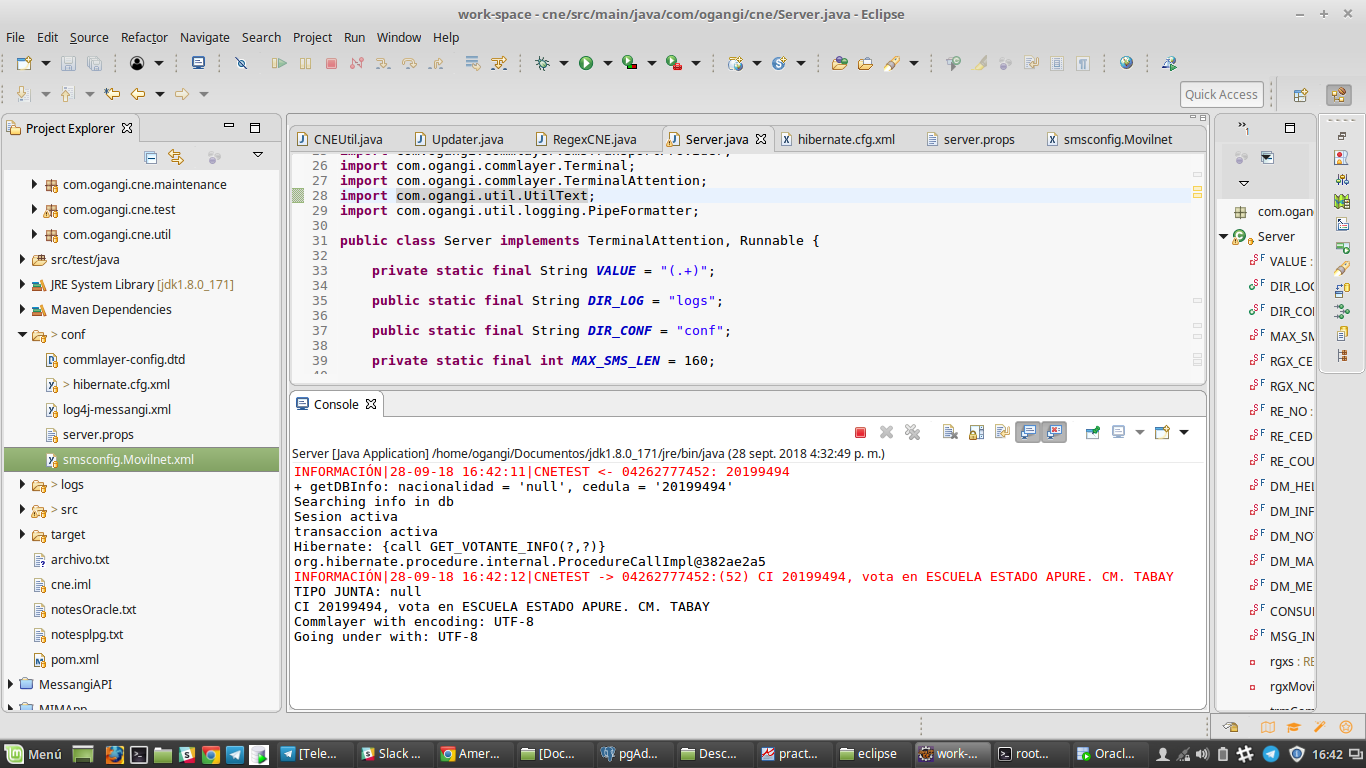
\includegraphics[width=0.8\textwidth]{recibido.png}
	\caption{Datos consultados por medio de los procedimientos almacenados}
	\label{l1}
\end{figure}

	\begin{figure}[H]
		\centering
		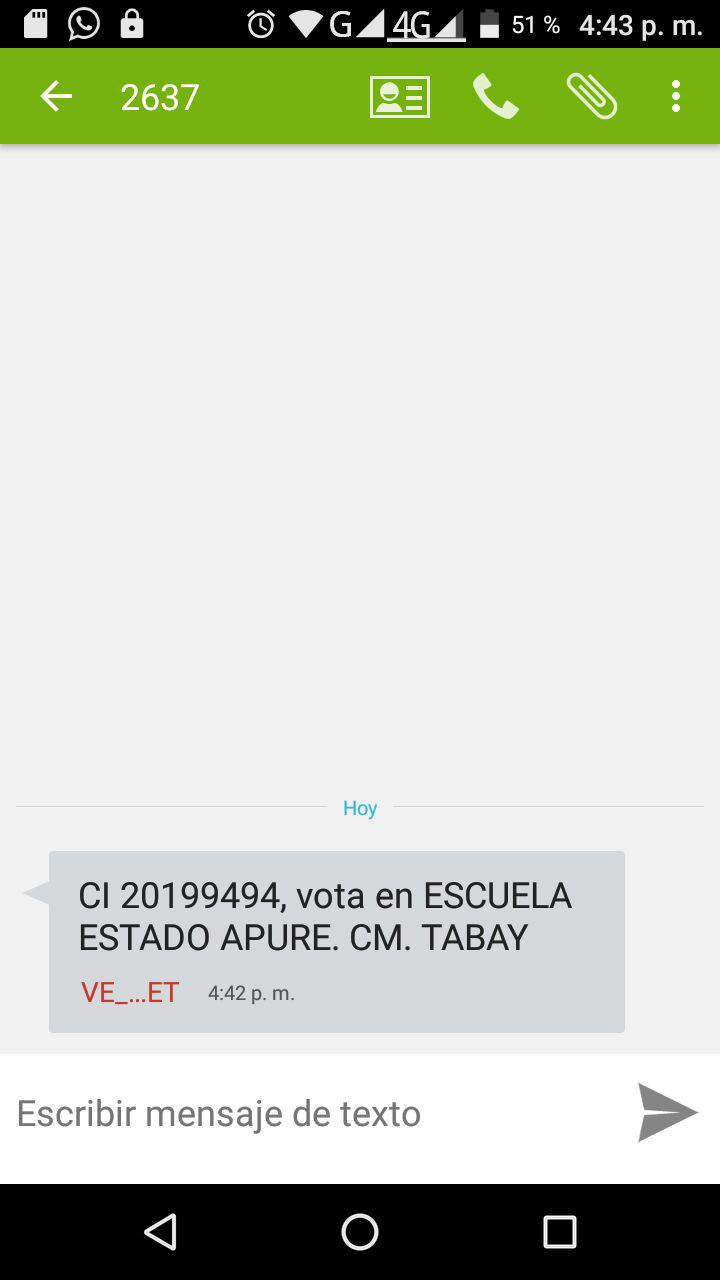
\includegraphics[width=0.3\textwidth]{pruebatlf.jpg}
		\caption{SMS recibido con los datos solicitados}
		\label{p1}
	\end{figure}

	
	\section{Vinculación del proyecto con las materias de la carrera}
	
	Para poder llevar a cabo el proyecto, fue necesario el uso de conocimientos teóricos y prácticos que han sido impartidos en el transcurso de la carrera. Uno de los mas importantes es el conocimiento adquirido de programación, donde se desarrolla la lógica para resolver este tipo de problemas.\\
	
	En el transcurso de la carrera se ven 3 programaciones, cada una con su nivel de dificultad. Para desarrollar este proyecto se necesito específicamente de los conocimientos aprendidos en Programación 2 y 3.\\
	
	En programación 2, se aprendió sobre el manejo de archivos y la programación orientada a Objetos. Este ultimo concepto es muy importante, ya que el lenguaje de programación utilizado para el desarrollo fue JAVA, el cual es un lenguaje de programación orientado a objetos.\\
	
	 El manejo de archivos fue necesario para guardar los datos extraídos de la base de datos en dichos documentos.\\
	
	En programación 3, se aprendió sobre estructuras de datos, ya que estas permiten organizar los datos de una manera eficiente, logrando así hacer un programa óptimo.\\
	
	Otros conceptos utilizados fueron los adquiridos en las materias del profesional, estas son: Base de Datos e Ingeniería del Software.\\
	
	En Base de Datos, se aprendió como diseñar de manera eficiente bases de datos relacionales. También como realizar la operaciones: insertar, modificar, eliminar y consultar a una Base de Datos.\\
	
	Otros de los conocimientos adquiridos, fue el de como manejar un Sistema de Gestor de Base De Datos, en este caso Postgresql, el cual es uno de los sistemas que esta siendo utilizado por la empresa.\\
	
	La creación y uso de los Procedimientos almacenados también se aprende en esta materia. Dichos procedimientos fueron muy utilizados en el proyecto.\\
	
	En ingeniería del Software, se enseñan los principios y las metodologías para el desarrollo y mantenimiento de sistemas software (Zelkovitz, 1978). En este proyecto se utilizo Scrum, la cual es una metodología ágil que se basa en una estructura de desarrollo incremental.
	
	\addcontentsline{toc}{chapter}{Conclusiones} 
	\chapter*{Conclusiones} 
	
	Comúnmente los estudiantes egresados de las universidades no han tenido la oportunidad de conocer el campo laboral para el que han sido formados, por esta razón realizar pasantías resulta una buena oportunidad para adquirir experiencia laboral y poder aplicar todo lo aprendido durante la carrera, guiado por un tutor empresarial el cual siempre ayudará al pasante en todo el periodo de duración de las mismas.\\
	
	El conocimiento adquirido te permite crecer profesionalmente y sentir mas seguridad a la hora de enfrentar el campo laboral. \\
	
	El principal objetivo del presente proyecto era optimizar el código del sistema y realizar el análisis, diseño e implementación de un módulo de Hibernate para el manejador de base de datos el cuál se logro completar satisfactoriamente, aplicando todos los conocimientos adquiridos en la carrera.\\
	
	Una acotación importante sería mejorar la base de datos utilizada por este proyecto ya que no cuenta con unas relaciones que permitan hacer las búsquedas de una manera eficiente.\\
	
	Realizar pasantías en Ogangi, es una experiencia gratificante ya que aparte de todos los conocimientos adquiridos, el ambiente de trabajo es muy agradable. Hay mucha unión y compañerismo y en cualquier situación en la que se necesite ayuda para realizar algún objetivo de un proyecto se puede contar con el apoyo de todos. \\
	
	Ogangi resulta ser una empresa en la cual la unión entre sus empleados hace que el trabajo sea mas agradable.
	% ***************************************************************** %
	% FIN DE
	% Agradecimientos y primer capitulo (sin numeracion)
	% ***************************************************************** %
	

	% ***************************************************************** %
	% Cuerpo
	% ***************************************************************** %
	
	%\input{capitulo1}
	%\input{capitulo2}
	%\input{capitulo3}
	%\input{capitulo4}
	%\input{capitulo5}
	

\addcontentsline{toc}{chapter}{Bibliografías} 

\begin{thebibliography}{9}
	\bibitem {lamport94}
	Wikilibros(2014)
	\textit{ Programación Orientada a Objetos}, \\
	 https://es.wikibooks.org/wiki/Programación\_Orientada\_a\_Objetos
	
	\bibitem{revista}
	Revista Digital \textit{INESEM}
	\textit{Los gestores de bases de datos más usados}, \\
	https://revistadigital.inesem.es/informatica-y-tics/los-gestores-de-bases-de-datos-mas-usados/
	
	\bibitem{Wikipedia1}
	Wikipedia(2018),
	\textit{Objeto(programación)}, \\
	https://es.wikipedia.org/wiki/Objeto\_(programación)\#Estado
	
		\bibitem{hibernate}
	educación IT blog(2013)
	\textit{¿Qué es Java Hibernate?}, \\
	http://blog.educacionit.com/2013/02/07/que-es-java-hibernate/
	
	
	\bibitem{Wikipedia2}
	Wikipedia(2017),
	\textit{Hibernate}, \\
	https://es.wikipedia.org/wiki/Hibernate
	
	
	\bibitem{Wikipedia3}
	Wikipedia(2018),
	\textit{Procedimiento almacenado}, \\
	https://es.wikipedia.org/wiki/Procedimiento\_almacenado
	
	\bibitem{definicion}
	Definicion,
	\textit{Definición de Java}, \\
	https://definicion.mx/java/
\end{thebibliography} 

	
 	
	% ***************************************************************** %
	% FIN DE
	% Cuerpo
	% ***************************************************************** %
	
	\addcontentsline{toc}{chapter}{Anexos} 
	\chapter*{Anexos}
	Las siguientes imágenes muestra código realizado por mi persona.
	\section{Creación de procedimientos Almacenados:}
	
	\begin{figure}[H]
		\centering
		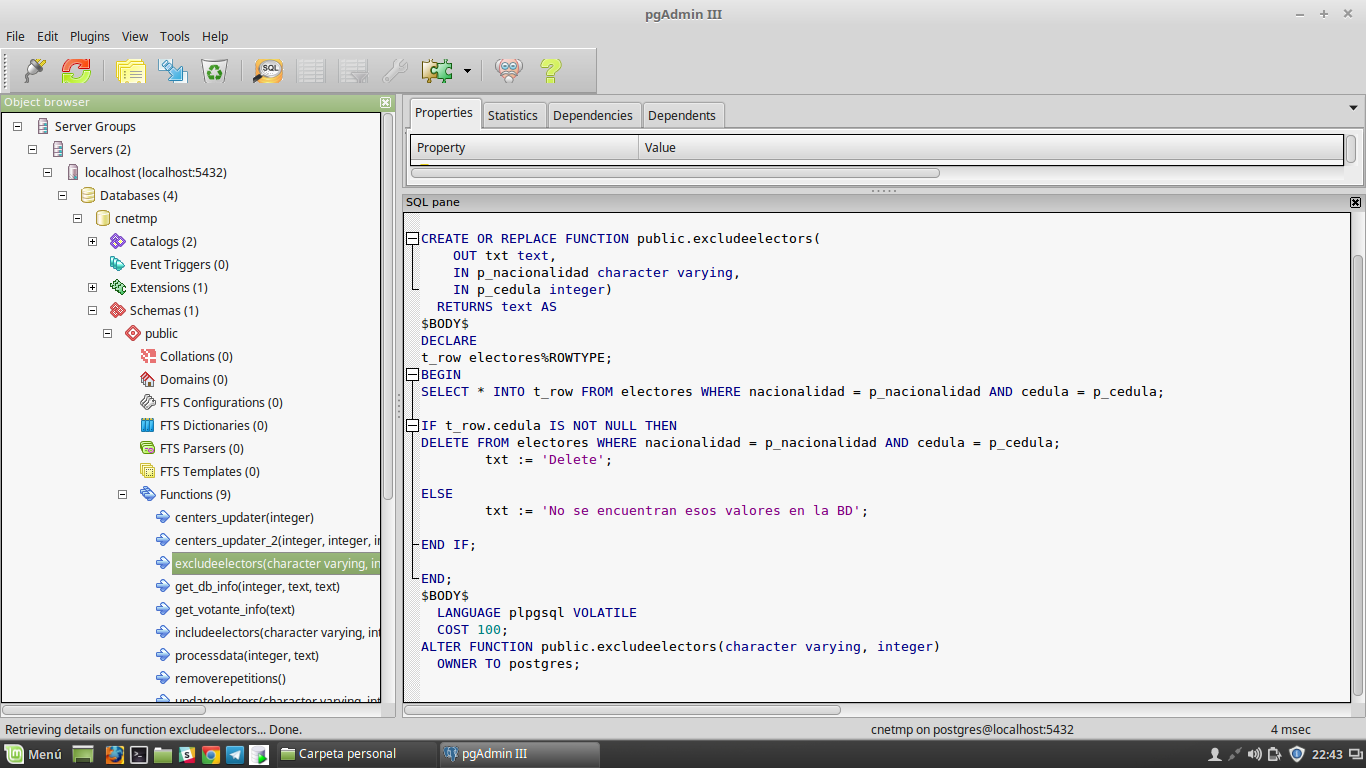
\includegraphics[width=0.8\textwidth]{excludeElector.png}
		\caption{Borra a un elector por medio de su cédula}
		\label{n1}
	\end{figure}

\begin{figure}[H]
	\centering
	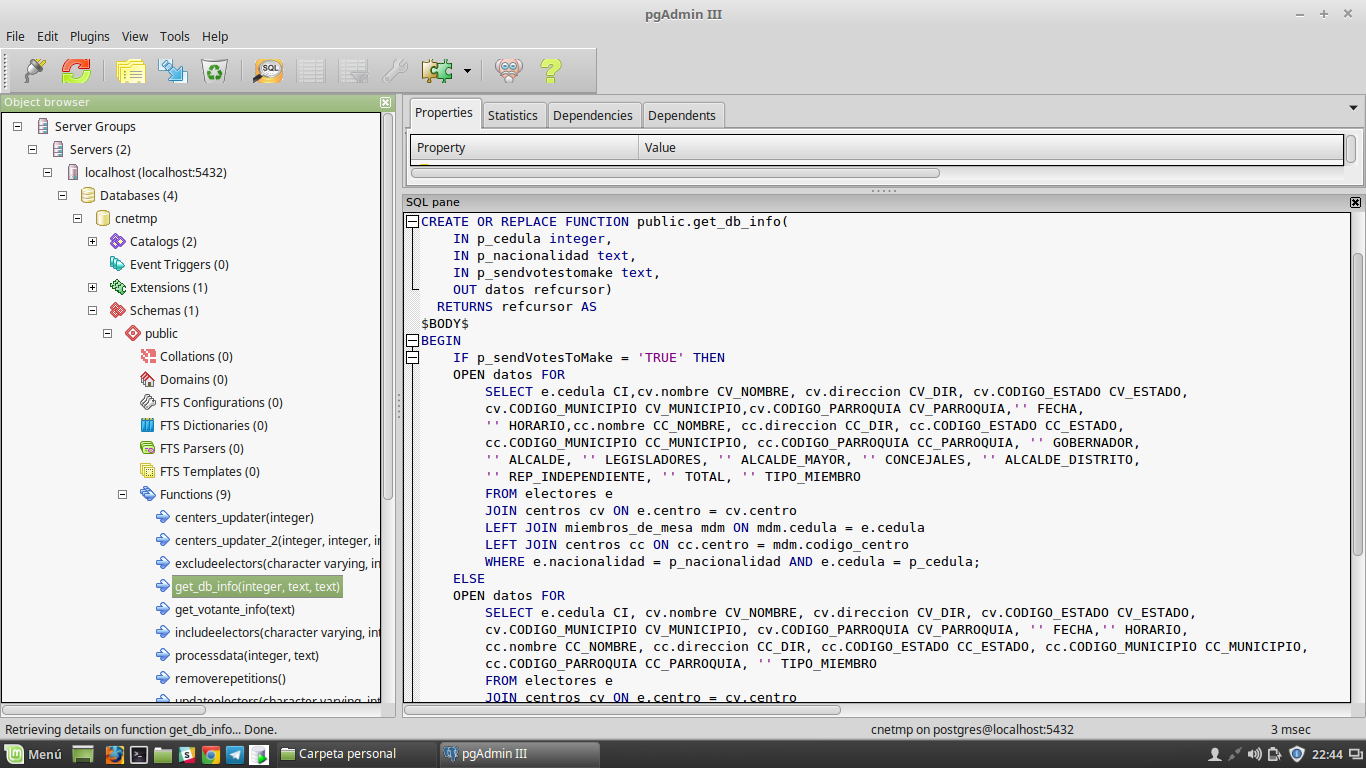
\includegraphics[width=0.8\textwidth]{get_db_info.png}
	\caption{Realiza una consulta diferente dependiendo de una condición}
	\label{m1}
\end{figure}

\begin{figure}[H]
	\centering
	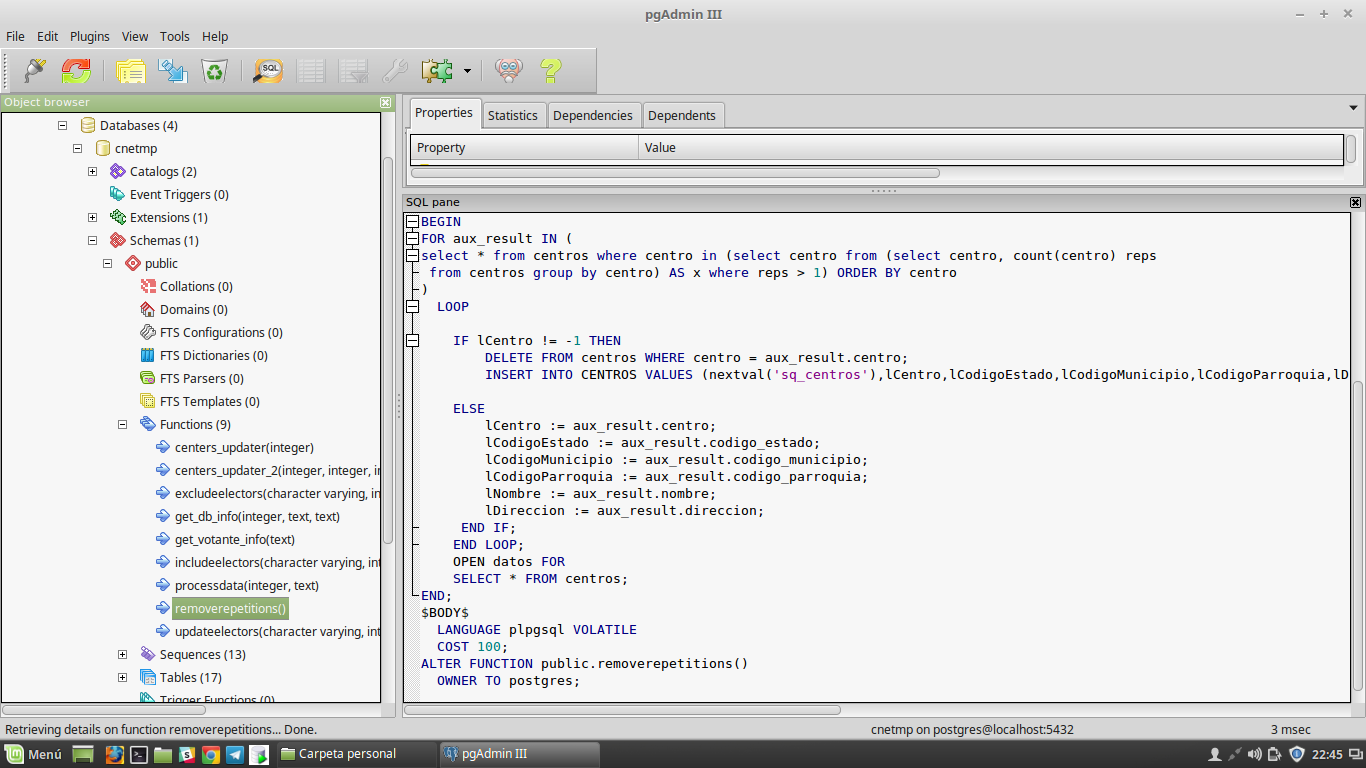
\includegraphics[width=0.8\textwidth]{remove_repetitions2.png}
	\caption{Elimina datos repetidos de una tabla y retorna el resultado}
	\label{o1}
\end{figure}
	
	\section{Llamados a los procedimientos almacenados:}

	\begin{figure}[H]
		\centering
		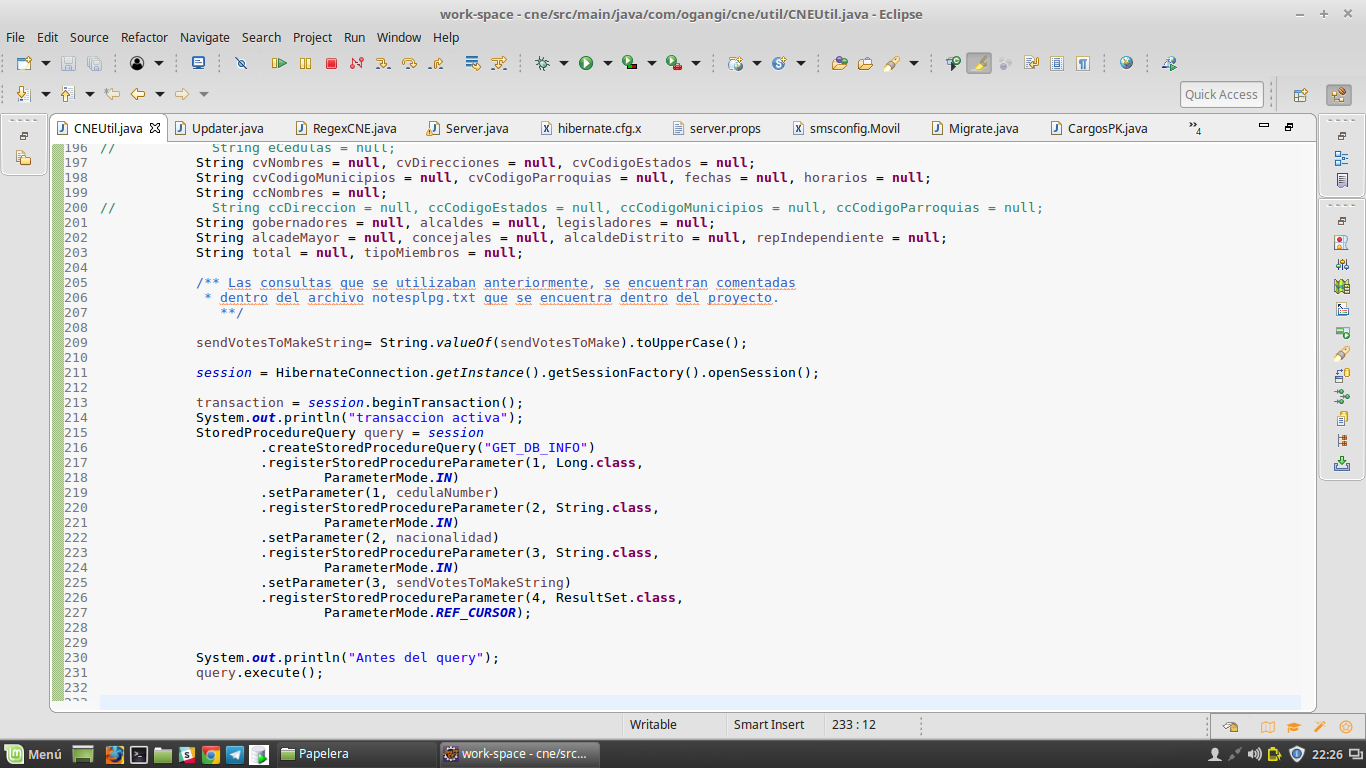
\includegraphics[width=0.8\textwidth]{getDataInfo().png}
		\caption{Llamado al procedimiento get\_data\_info()}
		\label{h1}
	\end{figure}
	
	\begin{figure}[H]
		\centering
		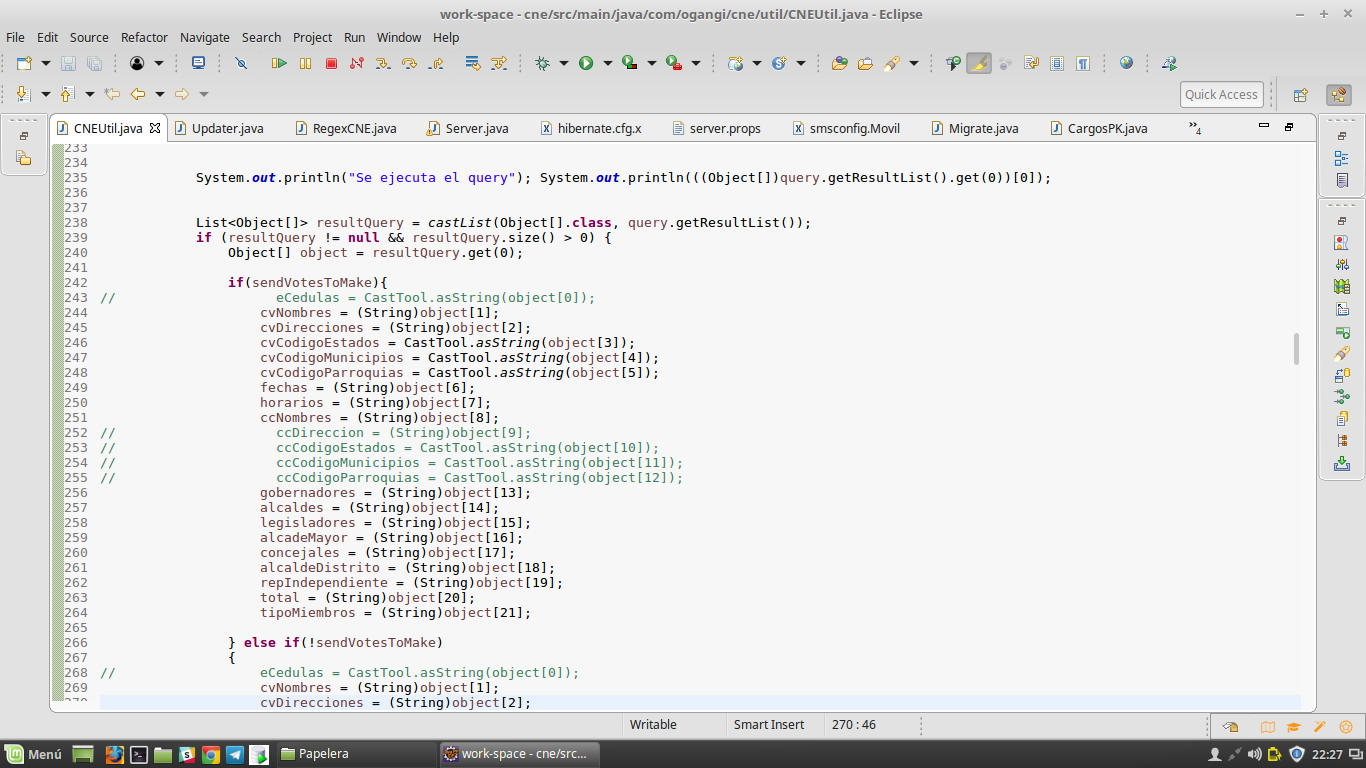
\includegraphics[width=0.8\textwidth]{getDataInfo2().png}
		\caption{El resultado del procedimiento se mostrara dependiendo de la condición que cumple }
		\label{b1}
	\end{figure}
	
	\section{Entidades en Hibernate:}
	
		\begin{figure}[H]
		\centering
		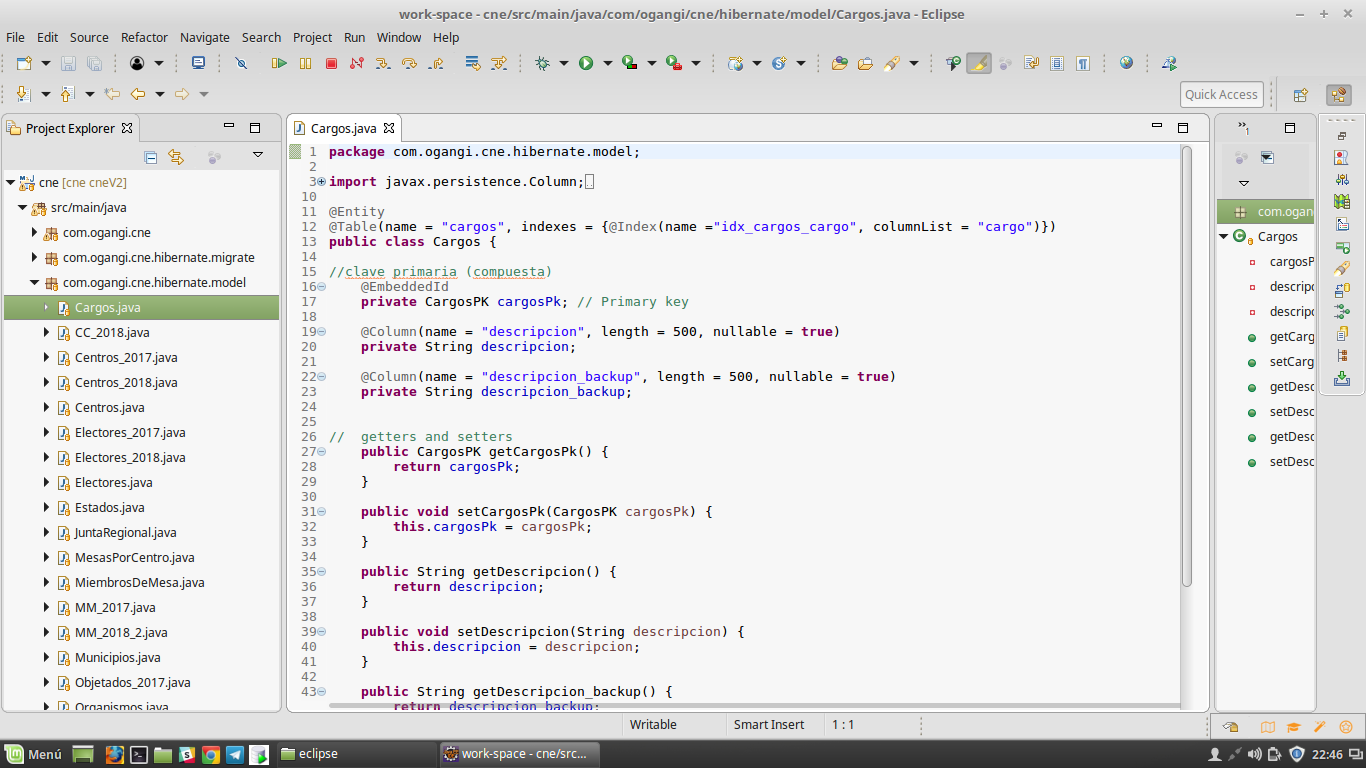
\includegraphics[width=0.8\textwidth]{cargos.png}
		\caption{Entidad que permite crear la tabla cargos}
		\label{k1}
	\end{figure}
	
	\begin{figure}[H]
		\centering
		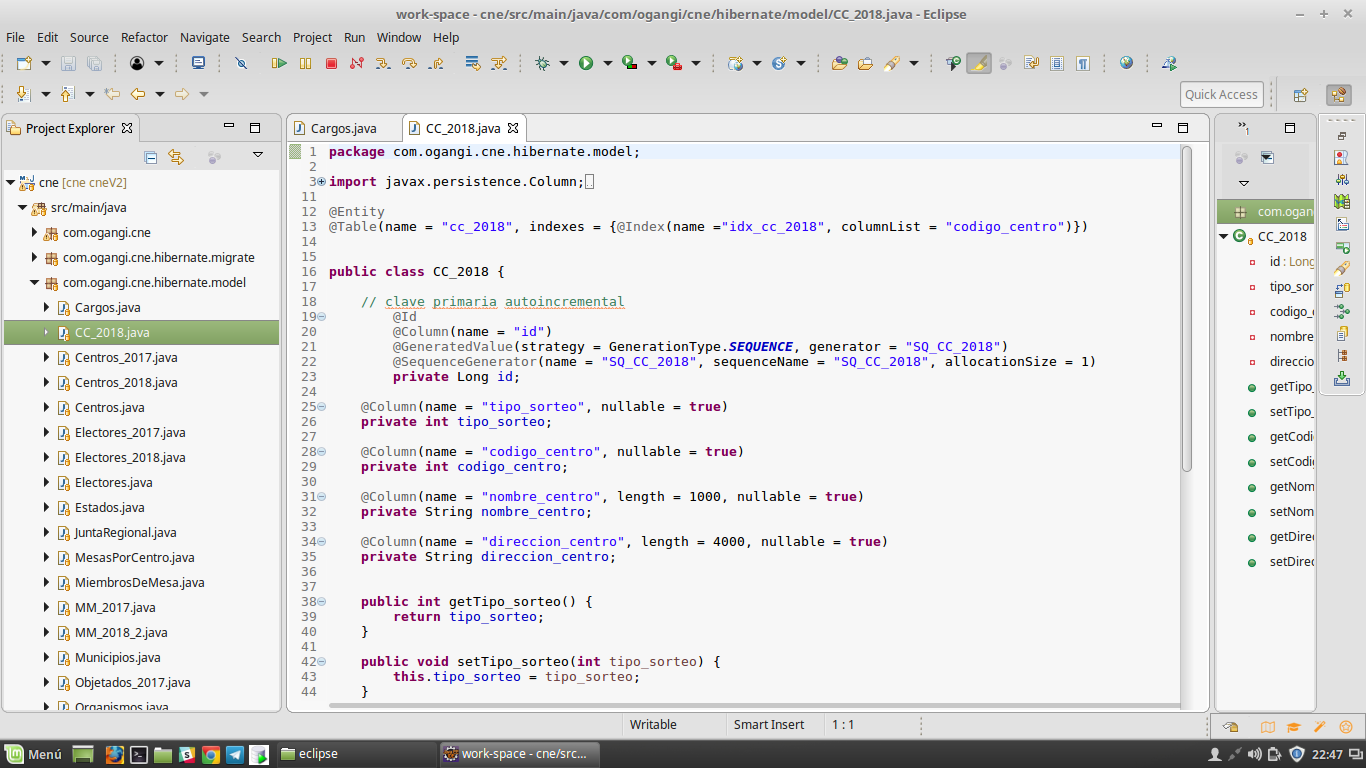
\includegraphics[width=0.8\textwidth]{cc_2018.png}
		\caption{Entidad que permite crear la tabla cc\_2018}
		\label{j1}
	\end{figure}
	
	\section{Archivo XML:}
	Este archivo se creó junto al tutor empresarial
	
		\begin{figure}[H]
		\centering
		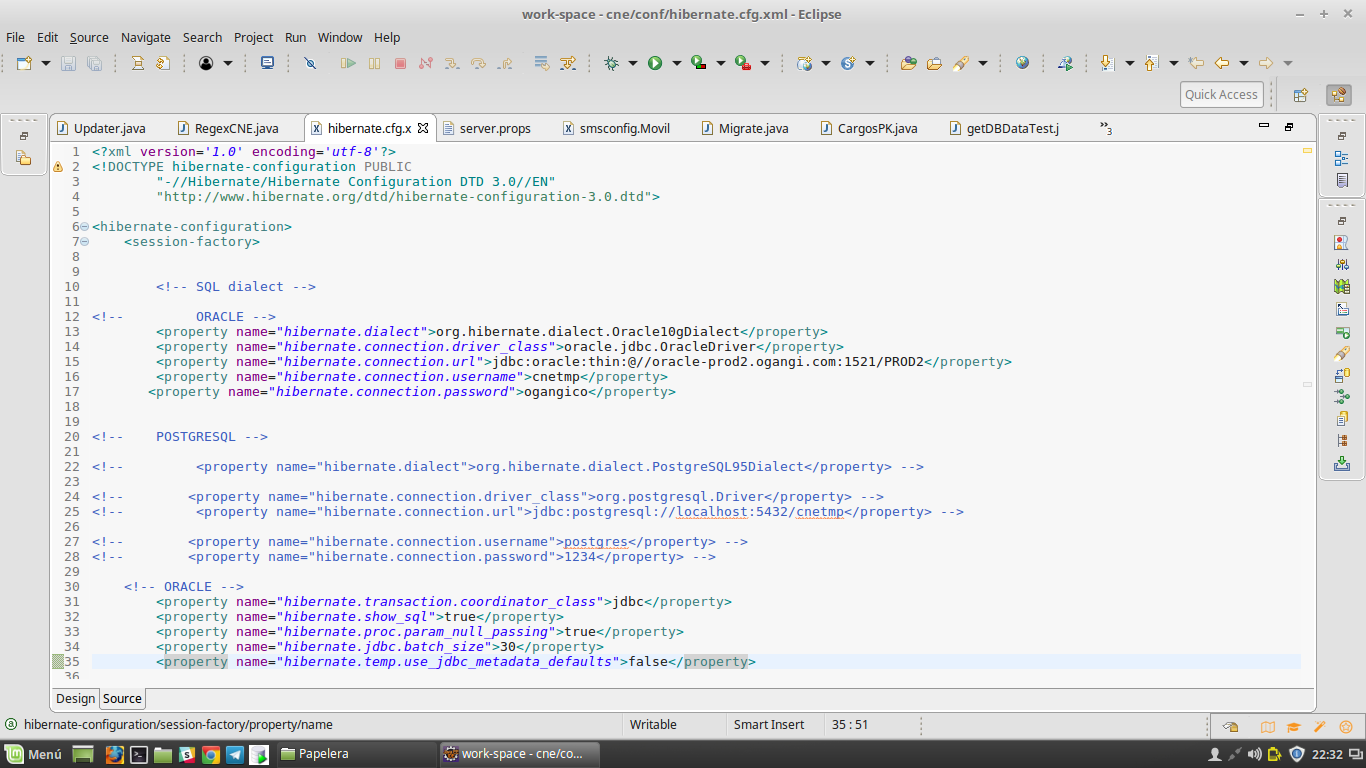
\includegraphics[width=0.8\textwidth]{hibernatexml.png}
		\caption{Se aprecia las conexiones a Oracle y Postgresql}
		\label{g1}
	\end{figure}
	
	\begin{figure}[H]
		\centering
		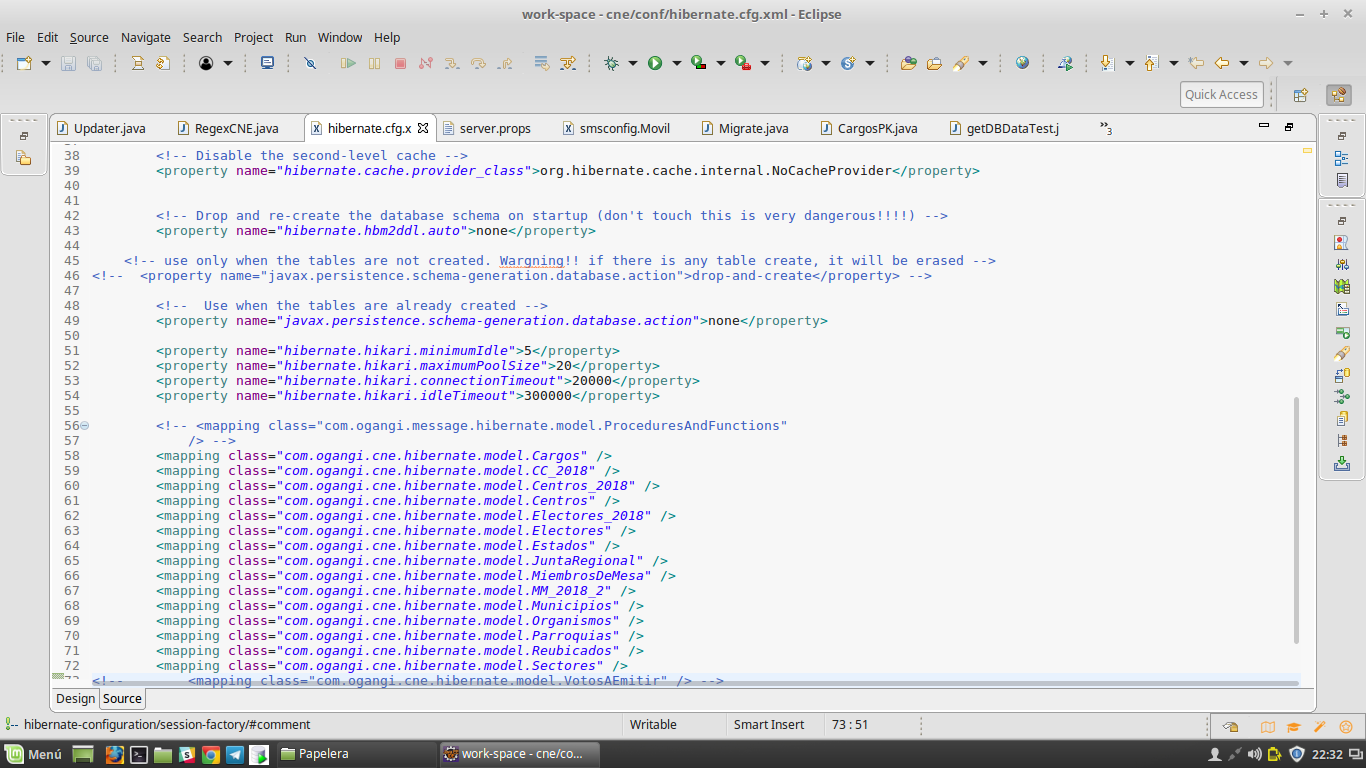
\includegraphics[width=0.8\textwidth]{hibernatexml2.png}
		\caption{Se aprecian todas las entidades que pueden ser creadas por Hibernate}
		\label{a1}
	\end{figure}

\section{Clase Migrate:}

Se mostrará algunos segmentos de una de las funciones del código de la clase migrate, la cual fue realizada por mi persona.

	\begin{figure}[H]
	\centering
	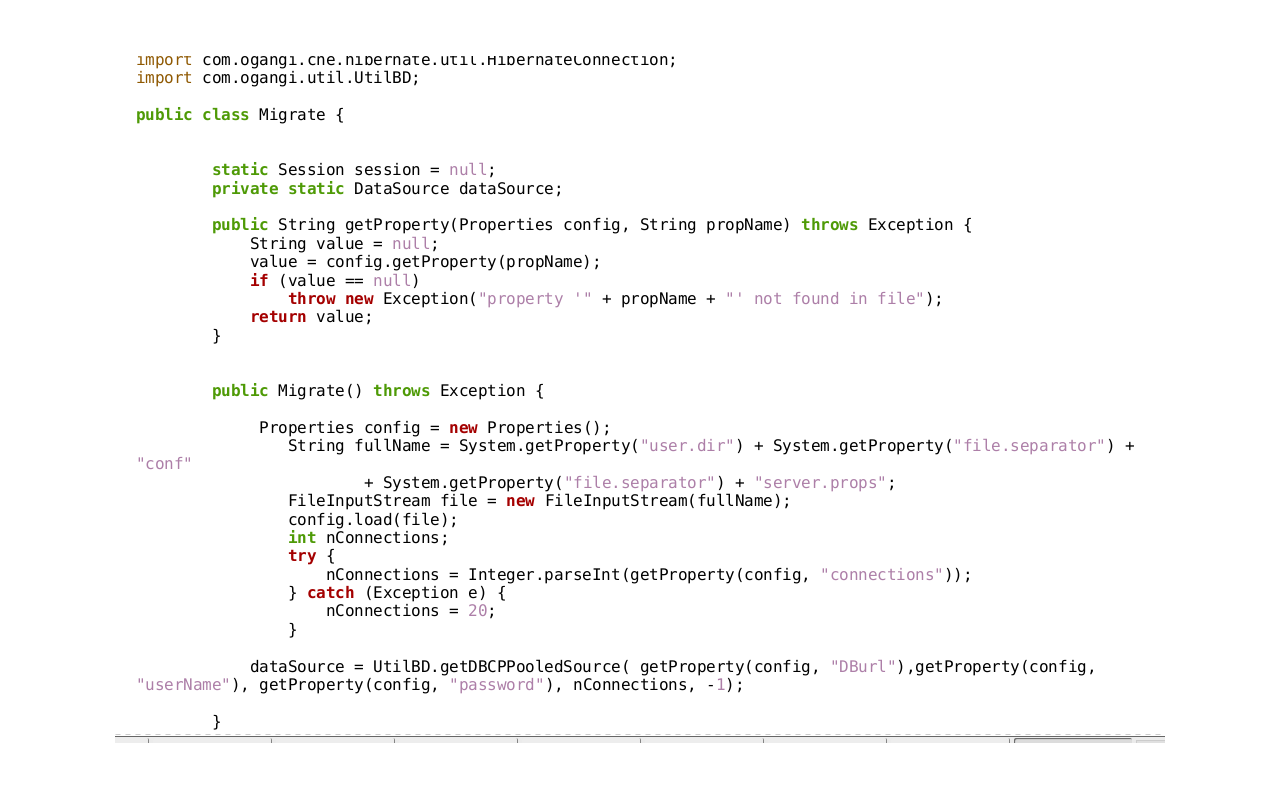
\includegraphics[width=0.8\textwidth]{migrate1.png}
	\caption{Se establece la conexión con Oracle y Postgresql}
	\label{q1}
\end{figure}

\begin{figure}[H]
	\centering
	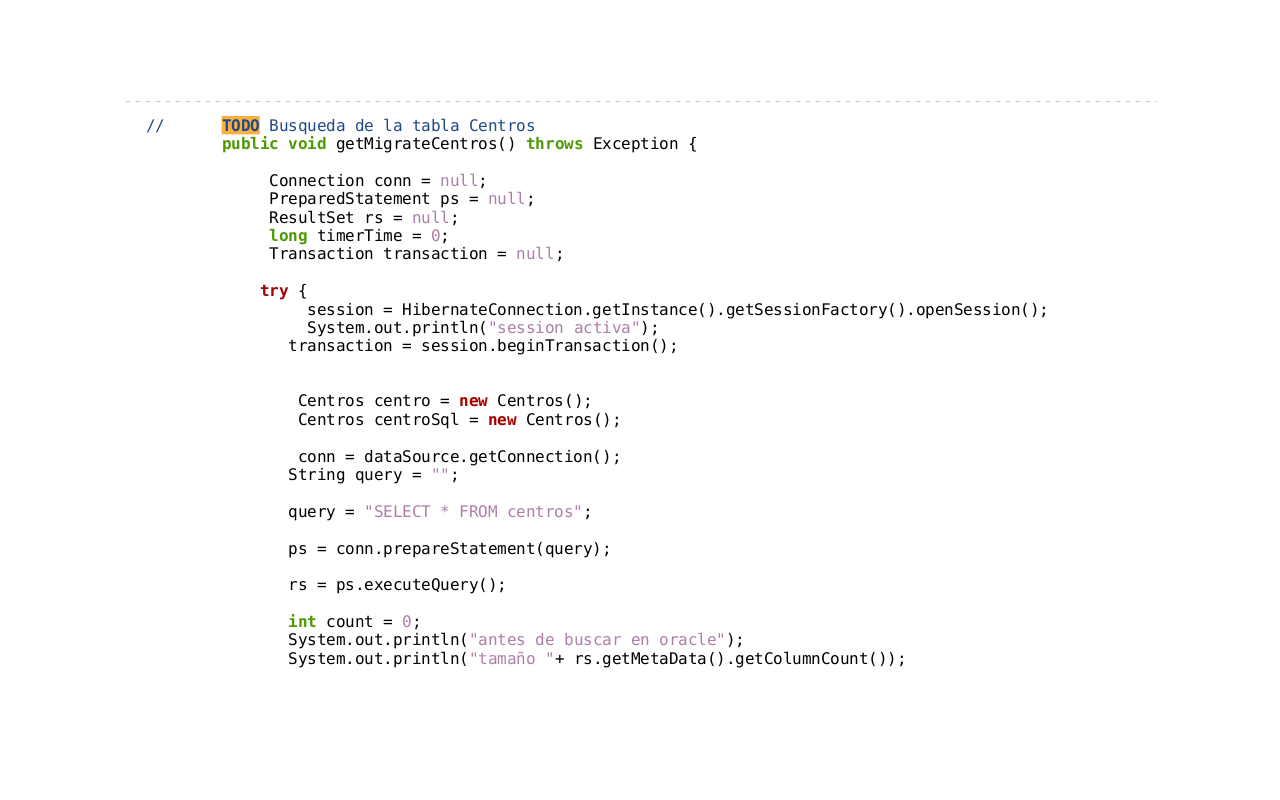
\includegraphics[width=0.8\textwidth]{migrate2.png}
	\caption{Función que permite la migración de Oracle a Postgresql}
	\label{e1}
\end{figure}

	\begin{figure}[H]
	\centering
	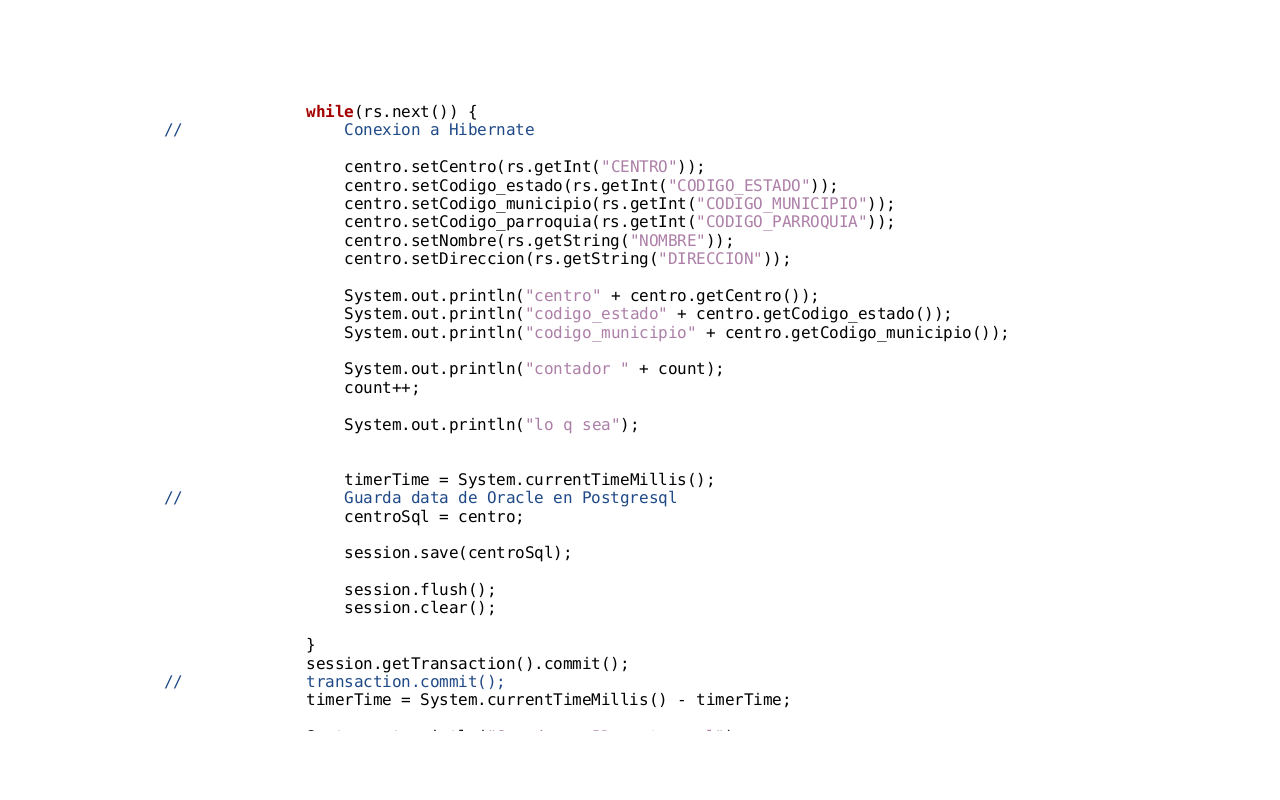
\includegraphics[width=0.8\textwidth]{migrate3.png}
	\caption{Guarda data de Oracle a Postgresql}
	\label{r1}
\end{figure}

\begin{figure}[H]
	\centering
	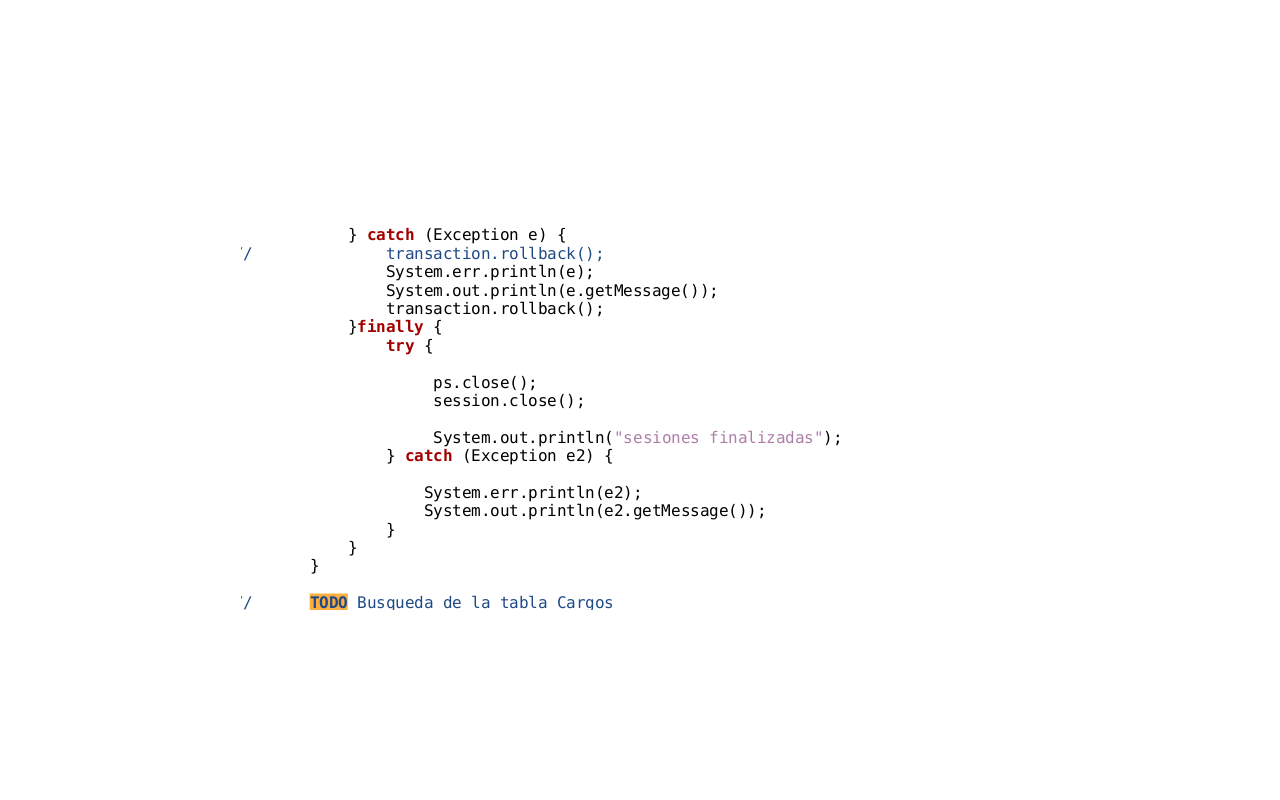
\includegraphics[width=0.8\textwidth]{migrate4.png}
	\caption{Finaliza la sesión}
	\label{t1}
\end{figure}

	% ***************************************************************** %
	% FIN DE
	% Cuerpo
	% ***************************************************************** %
	 
	\appendix
	\scriptsize

	
\end{document}
